\section*{The Database}



\begin{figure}
  \centering
  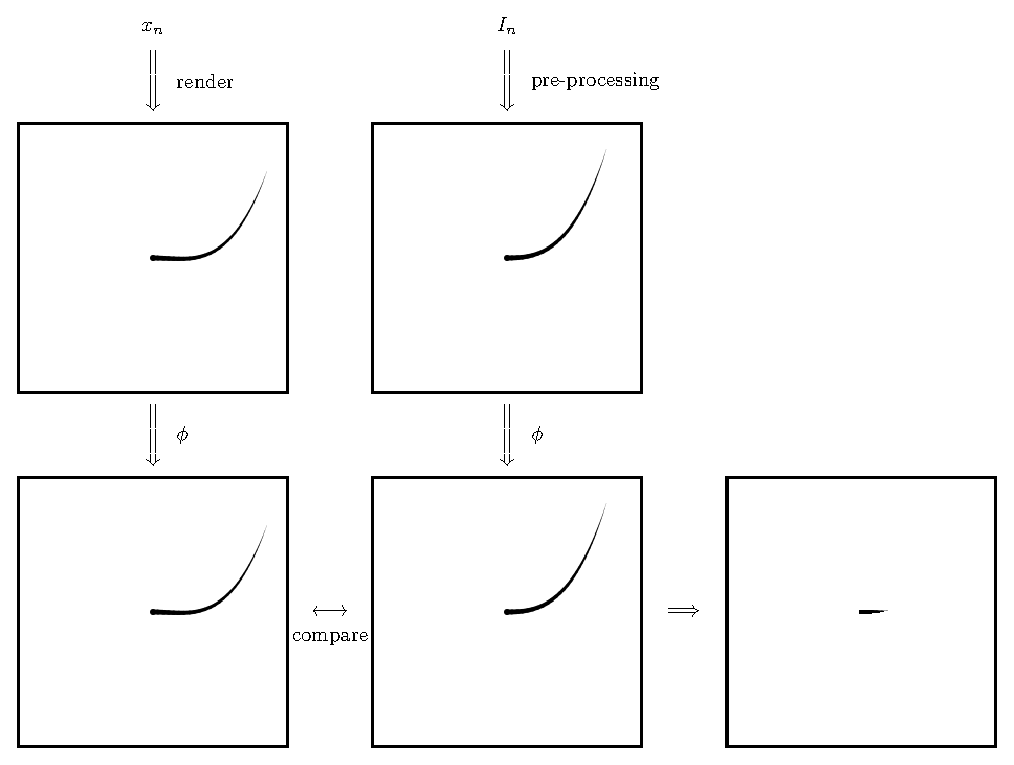
\includegraphics[scale=1.0]{whisker_compare.pdf}
  \caption{Schematic image of the process to evaluate importance of hypothesis.}
  \label{fig:whisker_compare}
\end{figure}

The $\phi$-transform is used to generate a sensory cue for the comparison, at the moment we have choosen to just use the identity transform since we have, compared to others, a homogeneous environment.

\begin{figure}
  \centering
  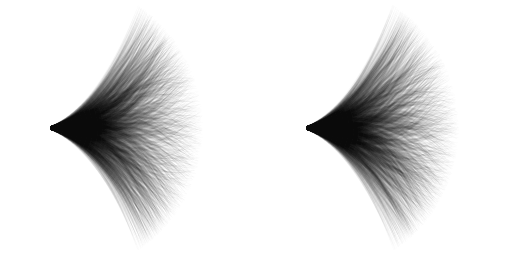
\includegraphics{database_gwhisker_spline3_n2048_from_to_fixed.png}
  \caption{View of all whiskers in transition database. Left: from-states. Right: to-states.}
  \label{fig:database}
\end{figure}
